


\tikzset{every picture/.style={line width=0.75pt}} %set default line width to 0.75pt        

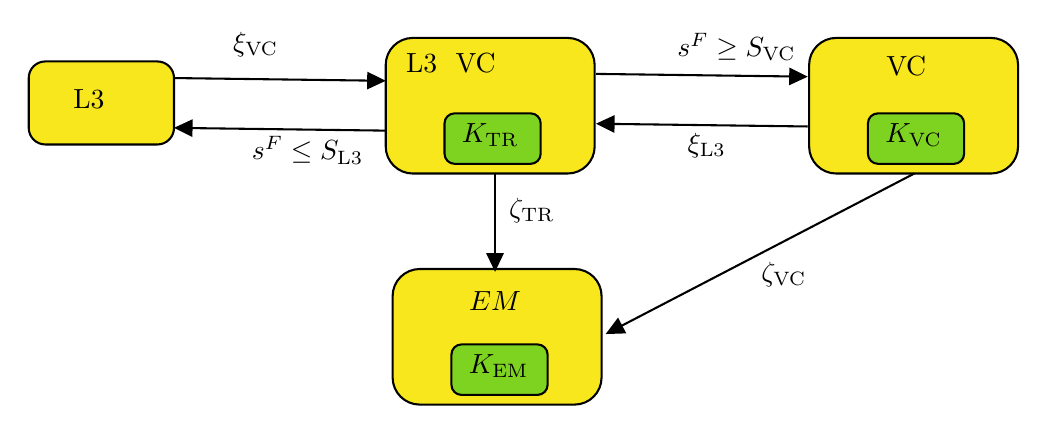
\begin{tikzpicture}[x=0.75pt,y=0.75pt,yscale=-1,xscale=1]
%uncomment if require: \path (0,300); %set diagram left start at 0, and has height of 300

%Rounded Rect [id:dp24689060389445716] 
\draw  [fill={rgb, 255:red, 248; green, 231; blue, 28 }  ,fill opacity=1 ] (105,135.67) .. controls (105,131.25) and (108.58,127.67) .. (113,127.67) -- (167,127.67) .. controls (171.42,127.67) and (175,131.25) .. (175,135.67) -- (175,159.67) .. controls (175,164.08) and (171.42,167.67) .. (167,167.67) -- (113,167.67) .. controls (108.58,167.67) and (105,164.08) .. (105,159.67) -- cycle ;
%Rounded Rect [id:dp03990125264398037] 
\draw  [fill={rgb, 255:red, 248; green, 231; blue, 28 }  ,fill opacity=1 ] (277,129.4) .. controls (277,122.18) and (282.85,116.33) .. (290.07,116.33) -- (364.6,116.33) .. controls (371.82,116.33) and (377.67,122.18) .. (377.67,129.4) -- (377.67,168.6) .. controls (377.67,175.82) and (371.82,181.67) .. (364.6,181.67) -- (290.07,181.67) .. controls (282.85,181.67) and (277,175.82) .. (277,168.6) -- cycle ;
%Rounded Rect [id:dp7956869543382266] 
\draw  [fill={rgb, 255:red, 126; green, 211; blue, 33 }  ,fill opacity=1 ] (305.33,157.53) .. controls (305.33,154.85) and (307.51,152.67) .. (310.2,152.67) -- (346.8,152.67) .. controls (349.49,152.67) and (351.67,154.85) .. (351.67,157.53) -- (351.67,172.13) .. controls (351.67,174.82) and (349.49,177) .. (346.8,177) -- (310.2,177) .. controls (307.51,177) and (305.33,174.82) .. (305.33,172.13) -- cycle ;

%Rounded Rect [id:dp9718527933811503] 
\draw  [fill={rgb, 255:red, 248; green, 231; blue, 28 }  ,fill opacity=1 ] (481,129.4) .. controls (481,122.18) and (486.85,116.33) .. (494.07,116.33) -- (568.6,116.33) .. controls (575.82,116.33) and (581.67,122.18) .. (581.67,129.4) -- (581.67,168.6) .. controls (581.67,175.82) and (575.82,181.67) .. (568.6,181.67) -- (494.07,181.67) .. controls (486.85,181.67) and (481,175.82) .. (481,168.6) -- cycle ;
%Rounded Rect [id:dp4375862505854522] 
\draw  [fill={rgb, 255:red, 126; green, 211; blue, 33 }  ,fill opacity=1 ] (509.33,157.53) .. controls (509.33,154.85) and (511.51,152.67) .. (514.2,152.67) -- (550.8,152.67) .. controls (553.49,152.67) and (555.67,154.85) .. (555.67,157.53) -- (555.67,172.13) .. controls (555.67,174.82) and (553.49,177) .. (550.8,177) -- (514.2,177) .. controls (511.51,177) and (509.33,174.82) .. (509.33,172.13) -- cycle ;

%Rounded Rect [id:dp876279933975634] 
\draw  [fill={rgb, 255:red, 248; green, 231; blue, 28 }  ,fill opacity=1 ] (280.33,240.73) .. controls (280.33,233.52) and (286.18,227.67) .. (293.4,227.67) -- (367.93,227.67) .. controls (375.15,227.67) and (381,233.52) .. (381,240.73) -- (381,279.93) .. controls (381,287.15) and (375.15,293) .. (367.93,293) -- (293.4,293) .. controls (286.18,293) and (280.33,287.15) .. (280.33,279.93) -- cycle ;
%Rounded Rect [id:dp039461928783934175] 
\draw  [fill={rgb, 255:red, 126; green, 211; blue, 33 }  ,fill opacity=1 ] (308.67,268.87) .. controls (308.67,266.18) and (310.85,264) .. (313.53,264) -- (350.13,264) .. controls (352.82,264) and (355,266.18) .. (355,268.87) -- (355,283.47) .. controls (355,286.15) and (352.82,288.33) .. (350.13,288.33) -- (313.53,288.33) .. controls (310.85,288.33) and (308.67,286.15) .. (308.67,283.47) -- cycle ;

%Straight Lines [id:da8518584621470304] 
\draw    (175,135.67) -- (274,136.96) ;
\draw [shift={(277,137)}, rotate = 180.75] [fill={rgb, 255:red, 0; green, 0; blue, 0 }  ][line width=0.08]  [draw opacity=0] (8.93,-4.29) -- (0,0) -- (8.93,4.29) -- cycle    ;
%Straight Lines [id:da31078013867281284] 
\draw    (178,159.71) -- (277,161) ;
\draw [shift={(175,159.67)}, rotate = 0.75] [fill={rgb, 255:red, 0; green, 0; blue, 0 }  ][line width=0.08]  [draw opacity=0] (8.93,-4.29) -- (0,0) -- (8.93,4.29) -- cycle    ;
%Straight Lines [id:da5622985546516415] 
\draw    (378.33,133.67) -- (477.33,134.96) ;
\draw [shift={(480.33,135)}, rotate = 180.75] [fill={rgb, 255:red, 0; green, 0; blue, 0 }  ][line width=0.08]  [draw opacity=0] (8.93,-4.29) -- (0,0) -- (8.93,4.29) -- cycle    ;
%Straight Lines [id:da8651290950592201] 
\draw    (381.33,157.71) -- (480.33,159) ;
\draw [shift={(378.33,157.67)}, rotate = 0.75] [fill={rgb, 255:red, 0; green, 0; blue, 0 }  ][line width=0.08]  [draw opacity=0] (8.93,-4.29) -- (0,0) -- (8.93,4.29) -- cycle    ;
%Straight Lines [id:da9169685244420764] 
\draw    (329.67,181.67) -- (329.67,226) ;
\draw [shift={(329.67,229)}, rotate = 270] [fill={rgb, 255:red, 0; green, 0; blue, 0 }  ][line width=0.08]  [draw opacity=0] (8.93,-4.29) -- (0,0) -- (8.93,4.29) -- cycle    ;
%Straight Lines [id:da5583832122874837] 
\draw    (531.67,181.67) -- (385.66,257.62) ;
\draw [shift={(383,259)}, rotate = 332.52] [fill={rgb, 255:red, 0; green, 0; blue, 0 }  ][line width=0.08]  [draw opacity=0] (8.93,-4.29) -- (0,0) -- (8.93,4.29) -- cycle    ;

% Text Node
\draw (125,139.73) node [anchor=north west][inner sep=0.75pt]    {$\mathrm{L3}$};
% Text Node
\draw (516.67,123.73) node [anchor=north west][inner sep=0.75pt]    {$\mathrm{VC}$};
% Text Node
\draw (516.2,156.07) node [anchor=north west][inner sep=0.75pt]    {$K_{\mathrm{VC}}$};
% Text Node
\draw (315.67,237.07) node [anchor=north west][inner sep=0.75pt]    {$EM$};
% Text Node
\draw (315.53,267.4) node [anchor=north west][inner sep=0.75pt]    {$K_{\mathrm{EM}}$};
% Text Node
\draw (312.2,156.07) node [anchor=north west][inner sep=0.75pt]    {$K_{\mathrm{TR}}$};
% Text Node
\draw (285.33,122.4) node [anchor=north west][inner sep=0.75pt]    {$\mathrm{L3}\ \rightleftarrows \ \mathrm{VC}$};
% Text Node
\draw (335,191.9) node [anchor=north west][inner sep=0.75pt]    {$\zeta _{\mathrm{TR}}$};
% Text Node
\draw (456.5,222.9) node [anchor=north west][inner sep=0.75pt]    {$\zeta _{\mathrm{VC}}$};
% Text Node
\draw (211,162.4) node [anchor=north west][inner sep=0.75pt]    {$s^F \leq S_{\mathrm{L3}}$};
% Text Node
\draw (416,112.4) node [anchor=north west][inner sep=0.75pt]    {$s^F \geq S_{\mathrm{VC}}$};
% Text Node
\draw (202,111.9) node [anchor=north west][inner sep=0.75pt]    {$\xi _{\mathrm{VC}}$};
% Text Node
\draw (421,160.9) node [anchor=north west][inner sep=0.75pt]    {$\xi _{\mathrm{L3} }$};


\end{tikzpicture}

